%----------------------------------------------------------------------------------------
%    SÈRIES DE TAYLOR I LAURENT
%----------------------------------------------------------------------------------------
\section{Sèries de Taylor i Laurent}
\subsubsection*{Sèrie geomètrica}
Considerem la sèrie geomètrica: $\displaystyle \sum_{k=0}^{n} z^{k} = 1 + z + z^{2} + \dots + z^{n} = \frac{1-z^{n+1}}{1-z}$, si $z \neq 1$. Quin comportament podem esperar de la sèrie quan $n \to \infty$?
\begin{align*}
    \sum_{k=0}^{\infty} z^{k} = \frac{1}{1 - z}, \quad \abs{z} < 1
\end{align*}
Aquest resultat és particularment útil, ja que ens servirà a càlculs posteriors.

%----------------------------------------------------------------------------------------
\subsection{Sèrie de Taylor}
\begin{thm}[de Taylor]
    Sigui $g(z)$ una funció analítica en un disc $\abs{z-z_{0}} < R_{0}$, centrat a $z_{0}$ i de radi $R_{0}$. Llavors, es compleix
    \begin{align}
        g(z) = \sum_{n=0}^{\infty} a_{n} (z-z_{0})^{n}, \quad \text{amb } a_{n} = \frac{g^{(n)}(z_{0})}{n!}
    \end{align}
\end{thm}
L'expansió en sèrie de $e^{z}$, $\sin z$, i $\cos z$ també tenen la mateixa forma que tenen a $\mbb{R}$:
\begin{itemize}
    \item $\displaystyle e^{z} = \sum_{n=0}^{\infty} \frac{z^{n}}{n!}$.
    \item $\displaystyle \sin z = \frac{e^{iz} - e^{-iz}}{2i} = \frac{1}{2i} \sum_{n=0}^{\infty} \frac{(iz)^{n} - (-iz)^{n}}{n!} = \sum_{n=0}^{\infty} \frac{(-1)^{n} z^{1+2n}}{(1+2n)!}$.
    \item $\displaystyle \cos z = \frac{e^{iz} + e^{-iz}}{2} = \frac{1}{2} \sum_{n=0}^{\infty} \frac{(iz)^{n} + (-iz)^{n}}{n!} = \sum_{n=0}^{\infty} \frac{(-1)^{n} z^{2n}}{(2n)!}$.
\end{itemize}

%----------------------------------------------------------------------------------------
\subsection{Sèrie de Laurent}
\begin{thm}[de Laurent]
	Sigui $g(z)$ una funció analítica a l'anell $\mc{R} = \lrcur{z \mid R_{1} < \abs{z - z_{0}} < R_{2}}$ centrat a $z_{0}$. Sigui $\mc{C}$ qualsevol camí tancat simple, orientat positivament, que rodeja a $z_{0}$ i $\mc{C} \subset \mc{R}$. Llavors, es compleix
	\begin{align}
		g(z) &= \sum_{n=0}^{\infty} a_{n} \lrpar{z-z_{0}}^{n} + \sum_{n=1}^{\infty} \frac{b_{n}}{\lrpar{z - z_{0}}}
	\end{align}
	amb $a_{n} = \dfrac{1}{2 \pi i} \displaystyle \int_{\mc{C}} \frac{g(z) \diff z}{\lrpar{z-z_{0}}^{n+1}}$, i $b_{n} = \dfrac{1}{2 \pi i} \displaystyle \int_{\mc{C}} \frac{g(z) \diff z}{\lrpar{z-z_{0}}^{-n+1}}$.

	O alternativament
	\begin{align}
		g(z) &= \sum_{n = -\infty}^{\infty} c_{n} \lrpar{z-z_{0}}^{n}
	\end{align}
	amb $c_{n} = \dfrac{1}{2\pi i} \displaystyle \int_{\mc{C}} \frac{g(z) \diff z}{\lrpar{z-z_{0}}^{n+1}}$.
\end{thm}

\begin{example}
    \begin{itemize}
        \item $\displaystyle f(z) = e^{z} = \sum_{n_{0}}^{\infty} \frac{z^{n}}{n!}$ (Taylor).
        \item $\displaystyle f(z) = e^{1/z} = \sum_{n_{0}}^{\infty} \frac{1}{z^{n}}\frac{1}{n!}$ (Laurent).
    \end{itemize}
    Com podem veure, l'estratègia per facilitar el càlcul de les sèries de Laurent és fer Taylor i fer el canvi de variable adequat.
\end{example}

%----------------------------------------------------------------------------------------
\subsection{Residu}
\begin{defi}[Residu]
	La constant $a_{-1}$ a la sèrie de Laurent de $f(z)$ al punt $z_{0}$ s'anomena residu de $f(z)$. Ho expressem de la següent forma:
	\begin{align}
	    \underset{z=z_{0}}{\operatorname{Res}} f(z) \equiv a_{-1}
    \end{align}
	Si $f(z)$ és analítica al punt $z_{0}$, el seu residu és zero; si $z_{0}$ és una singularitat, $\underset{z=z_{0}}{\operatorname{Res}} f(z) \neq 0$.
\end{defi}

\subsubsection*{Pol simple}
Fent Laurent, tenim $f(z) = \dfrac{a_{-1}}{z-z_{0}} +a_{0} + a_{1} + \dots$. Considerem la funció $g(z) = \lrpar{z-z_{0}} f(z)$, que és analítica, per tant podem fer Taylor: $g(z) = a_{-1} + a_{0}\lrpar{z-z_{0}} + a_{1}\lrpar{z-z_{0}}^{2}$. Així doncs,
\begin{align}
	\underset{z=z_{0}}{\operatorname{Res}} f(z) = \lim_{z \to z_{0}} \lrpar{z-z_{0}} f(z)
\end{align}

\subsubsection*{Pol d'ordre $n$}
Fent Laurent, tenim $f(z) = \dfrac{a_{-n}}{\lrpar{z-z_{0}}^{n}} + \dfrac{a_{n-1}}{\lrpar{z-z_{0}}^{n-1}} + \dots + \dfrac{a_{-1}}{\lrpar{z-z_{0}}} + a_{0} + a_{1}\lrpar{z-z_{0}}$. Considerem la funció $g(z) = \lrpar{z-z_{0}}^{n} f(z)$, que és analítica, per tant podem fer Taylor: $ g(z) = \displaystyle \sum_{s=0}^{\infty} \dfrac{g^{s}(z_{0}) \lrpar{z-z_{0}}}{s!}$. Així doncs,
\begin{align}
	\underset{z=z_{0}}{\operatorname{Res}} f(z) = \lim_{z \to z_{0}} \frac{1}{(n-1)!} \der[n-1]{}{z} \lrbra{\lrpar{z-z_{0}}^{n} f(z)}
\end{align}

\begin{thm}[del residu]
	Si $\mc{C}$ és una corba tancada simple, orientada positivament, i $f(z)$ és analítica al seu interior excepte per un nombre finit de singularitats aïllades $z_{j}$ dins de $\mc{C}$ i un nombre finit de pols simples $z_{s}$ a la corba. Llavors, es compleix
	\begin{align}
		\int_{\mc{C}'} f(z) \diff z = 2\pi i \sum_{j=1}^{n} \underset{z=z_{j}}{\operatorname{Res}} f(z) + \pi i \sum_{s=1}^{m} \underset{z=z_{s}}{\operatorname{Res}} f(z)
	\end{align}
	on $\mc{C}' = \mc{C}\backslash \lrcur{\text{punts singulars } z_{s}}$.
\end{thm}

% \begin{lem}[dels arcs petits]
% \end{lem}

%----------------------------------------------------------------------------------------
\subsection{Càlcul d'integrals reals}
\subsubsection*{Integrals racionals trigonomètriques}
Sigui $G(\sin \theta, \cos \theta)$ una funció racional trigonomètrica. Llavors, la integral de $G(\theta) \mid \theta \in [0,2\pi]$ és
\begin{align}
    \int_{0}^{2\pi} G(\sin \theta, \cos \theta) \diff \theta = \oint_{\mc{C}} G\lrpar{\frac{1}{2}\lrbra{z + \frac{1}{z}}, \frac{1}{2i}\lrbra{z - \frac{1}{z}}} \frac{\dif \theta}{iz}
\end{align}
\begin{sproof}
    Fent el canvi $z = e^{i\theta} \Rightarrow \displaystyle \frac{1}{z} = e^{-i\theta}$, arribem a $\displaystyle \cos \theta = \frac{1}{2}\lrpar{z + \frac{1}{z}}$ i $\displaystyle \sin \theta = \frac{1}{2i}\lrpar{z - \frac{1}{z}}$.
\end{sproof}

\subsubsection*{Estudi dels pols simples}
Sigui $G(\theta) = \dfrac{\dif \theta}{a + b \cos \theta}$ una funció trigonomètrica racional. Llavors, podem expressar la integral sobre la corba $\abs{z} = 1$ com
\begin{align}
    \int_{0}^{2\pi} \frac{\dif \theta}{a + b \cos \theta} = \frac{2}{ib} \int_{\abs{z} = 1} \frac{\dif z}{z^{2} + 2Az + 1}, \quad \text{amb } A = \frac{a}{b}
\end{align}

\begin{sproof}
	$\displaystyle \int_{0}^{2\pi} \frac{\dif \theta}{a + b \cos \theta} = \int_{\abs{z} = 1} \frac{\dif z}{iz \lrpar{a + b \frac{z^{2}+1}{2z}}} = \frac{1}{ib} \int_{\abs{z} = 1} \frac{\dif z}{\frac{z^{2} + 1}{2} + Az} = \frac{2}{ib} \int_{\abs{z} = 1} \frac{\dif z}{z^{2} + 2Az + 1}$.
\end{sproof}
Així doncs, segons la naturalesa dels pols que tingui la funció, la seva integral tindrà un resultat o un altre. En concret, veiem que són els següents:
\begin{align}
    \int_{0}^{2\pi} \frac{\dif \theta}{a + b \cos \theta} = \begin{cases} \dfrac{2\pi}{\sqrt{a^{2} - b^{2}}}, & \lrpar{\dfrac{a}{b}}^{2} > 1 \\ 0, & \lrpar{\dfrac{a}{b}}^{2} < 1 \end{cases}
\end{align}
\begin{sproof}
    Fent $z^{2} + 2Az + 1 = 0$ trobem el següents pols simples:
    \begin{itemize}
    	\item $A^{2} > 1: z_{\pm} = -A \pm \sqrt{A^{2} -1}$.
    	    \newline $\displaystyle \dfrac{2}{ib} \int \dfrac{\dif z}{(z - z_{+})(z - z_{-})} = \dfrac{2}{ib} (2\pi i) \underset{z = z_{+}}{\operatorname{Res}} \dfrac{\dif z}{z^{2} + 2Az + 1}$
    	    \newline $\displaystyle \phantom{\dfrac{2}{ib} \int \dfrac{\dif z}{(z - z_{+})(z - z_{-})}} = \frac{2}{ib} (2\pi i) \dfrac{1}{2z_{+} + 2z{-}} = \dfrac{2\pi}{\sqrt{a^{2} - b^{2}}}$.
    	\item $A^{2} < 1: z_{\pm} = -A \pm i \sqrt{1 - A^{2}} \Rightarrow \abs{z_{\pm}} = 1$.
        	\newline Fem $a + b \cos \theta = 0 \Rightarrow \cos \theta = -\dfrac{a}{b} = - \sqrt{A} < 1$. Llavors, tenim una integral impròpia amb pols simples a la corba, i tenim
        	\newline $\displaystyle \int_{0}^{2\pi} \frac{\dif \theta}{a + b \cos \theta} = \int_{\mc{C}_{A}} \frac{\dif z}{z^{2} + 2Az + 1} = - \int_{\mc{C}_{1}} - \int_{\mc{C}_{2}}$
        	\newline $\displaystyle \phantom{\int_{0}^{2\pi} \frac{\dif \theta}{a + b \cos \theta}} = - \dfrac{\pi}{2i\sqrt{1-A^{2}}} + \dfrac{\pi}{2i \sqrt{1-A^{2}}} \equiv 0$.
    \end{itemize}
\end{sproof}

\begin{example}
    $\displaystyle \int_{0}^{2\pi} \frac{\dif \theta}{2 + \cos \theta} = -i \oint_{\abs{z}=1} \frac{2 \diff z}{z^{2} + 4z + 1} \Rightarrow$ les singularitats són $z = -2 \pm \sqrt{3}$, llavors,
    \begin{align*}
    \begin{aligned}
        \int_{0}^{2\pi} \frac{\dif \theta}{2 + \cos \theta} &= -i (2\pi i) \underset{z=-2+\sqrt{3}}{\operatorname{Res}} \lrpar{\frac{2}{z^{2} + 4z + 1}} \\
        &= \lim_{z\to -2 + \sqrt{3}} \lrbra{\lrpar{z + 2 - \sqrt{3}} \lrpar{\frac{2}{z^{2} + 4z + 1}}} \\
        &= \eval{\frac{4\pi}{2z + 4}}_{z = -2 + \sqrt{3}} = \frac{2\pi}{\sqrt{3}} = \frac{2\pi}{\sqrt{2^{2} - 1^{2}}}
    \end{aligned}
    \end{align*}
\end{example}
%--------------
\subsubsection*{Integrals reals racionals de polinomis reals}
Siguin $P(x)$ i $Q(x)$ dues funcions reals tals que $\deg{P(x)} + 2 \leq \deg{Q(x)}$. Llavors, la integral de $\dfrac{P(x)}{Q(x)} \mid x \in (-\infty, \infty)$ és
\begin{align}
    \int_{-\infty}^{\infty} \frac{P(x)}{Q(x)} \diff x = 2\pi i \sum_{\operatorname{Im}z_{j} > 0} \underset{z=z_{j}}{\operatorname{Res}} \lrpar{\frac{P(z)}{Q(z)}} + \pi i \sum_{\operatorname{Im}z_{s} > 0} \underset{z=z_{s}}{\operatorname{Res}} \lrpar{\frac{P(z)}{Q(z)}}
\end{align}
on $z_{j}$ són singularitats aïllades dins la regió tancada per la corba d'integració i $z_{s}$ pols simples a la recta real $\mbb{R}$.

\begin{figure}[H]
    \centering
    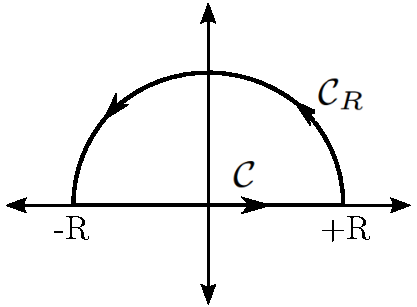
\includegraphics[width=0.3\textwidth]{./images/graph51}
    \caption{Representació gràfica dels camins sobre els quals s'integra la funció $\dfrac{P(x)}{Q(x)}$ a la demostració}
    \label{fig:graph51}
\end{figure}

\begin{sproof}
    \begin{align*}
    \begin{aligned}
        \int_{\mc{C} + \mc{C}_{R}} \frac{P(z)}{Q(z)} \diff z &= 2\pi i \sum_{\operatorname{Im}z_{j} > 0} \underset{z=z_{j}}{\operatorname{Res}} \frac{P(z)}{Q(z)} + \pi i \sum_{\operatorname{Im}z_{s} > 0} \underset{z=z_{s}}{\operatorname{Res}} \frac{P(z)}{Q(z)} \\
        &= \int_{\mc{C}} + \int_{\mc{C}_{R}} = I + I_{R}
    \end{aligned}
    \end{align*}
    Obserevem que volem trobar el valor de $I =\int_{\mc{C}} \frac{P(x)}{Q(x)} \diff x$. Fent la parametrització $z = R e^{i\theta} \Rightarrow$
    \begin{itemize}
        \item $\displaystyle \abs{I_{R}} \leq \int_{0}^{\pi} \abs{\frac{P\lrpar{Re^{i\theta}}}{Q\lrpar{Re^{i\theta}}}} R \diff \theta = \int_{0}^{\pi} \frac{\abs{z}^{m} + \dots }{\abs{z}^{m+s} + \dots} R \diff \theta = \pi \frac{R^{m+1}}{R^{m+s}} \underset{R \to 0}{\longrightarrow} 0$.
    \end{itemize}
    Llavors, tenim $\displaystyle I = \int_{\mc{C} + \mc{C}_{R}} \frac{P(z)}{Q(z)} \diff x$.
\end{sproof}

%--------------
\subsubsection*{Integrals reals racionals afegint una fase}
Siguin $P(x)$ i $Q(x)$ dues funcions reals tals que $\deg{P(x)} + 2 \leq \deg{Q(x)}$. Llavors, la integral de $\dfrac{P(x)}{Q(x)} e^{ix} \mid x \in (-\infty, \infty)$ és
\begin{align}
\begin{aligned}
    \int_{-\infty}^{\infty} \frac{P(x)}{Q(x)} e^{ix} \diff x &= 2\pi i \sum_{\operatorname{Im}z_{j} > 0} \underset{z=z_{j}}{\operatorname{Res}} \lrpar{\frac{P(z)}{Q(z)} e^{iz}} \\
    &+ \pi i \sum_{\operatorname{Im}z_{s} > 0} \underset{z=z_{s}}{\operatorname{Res}} \lrpar{\frac{P(z)}{Q(z)} e^{iz}}
\end{aligned}
\end{align}
on $z_{j}$ són singularitats aïllades dins la regió tancada per la corba d'integració i $z_{s}$ pols simples a la recta real $\mbb{R}$.

\begin{sproof}
    \begin{align*}
    \begin{aligned}
        \int_{\mc{C} + \mc{C}_{R}} \frac{P(z)}{Q(z)} e^{iz} \diff z &= 2\pi i \sum_{\operatorname{Im}z_{j} > 0} \underset{z=z_{j}}{\operatorname{Res}} \lrpar{\frac{P(z)}{Q(z)} e^{iz}} + \pi i \sum_{\operatorname{Im}z_{s} > 0} \underset{z=z_{s}}{\operatorname{Res}} \lrpar{\frac{P(z)}{Q(z)} e^{iz}} \\
        &= \int_{\mc{C}} + \int_{\mc{C}_{R}} = I + I_{R}
    \end{aligned}
    \end{align*}
    Obserevem que volem trobar el valor de $I =\int_{\mc{C}} \frac{P(x)}{Q(x)} e^{ix} \diff x$.
    \begin{itemize}
        \item $I_{R} = 0$, pel lema de Jordan.
    \end{itemize}
    Llavors, tenim $\displaystyle I = \int_{\mc{C} + \mc{C}_{R}} \frac{P(z)}{Q(z)} e^{iz} \diff x$.
\end{sproof}

\begin{lem}[de Jordan]
    Sigui $g(z)$ una funció analítica tal que $\displaystyle \lim_{\abs{z}\to \infty} \abs{g(z)} = 0$, i que $\operatorname{Im} z \geq 0$. Llavors, es compleix
    \begin{align}
        \int_{\mc{C}_{R}} g(z) e^{imz} \diff z \underset{R \to \infty}{\longrightarrow} 0, \quad m > 0
    \end{align}
\end{lem}
\begin{sproof}
    $e^{imz} = e^{imR(\Cos \theta + i \Sin \theta)} = e^{-mR\Sin \theta} e^{imR\Cos \theta}$. Observem que $e^{-mR\Sin \theta} \geq 0$ quan $\theta \in [0,\pi]$, i que $e^{imR\Cos \theta}$ no és més que una fase.

    Llavors, $\displaystyle \abs{I} \equiv \abs{\int_{\mc{C}} g(z) e^{imz} \diff z} \leq \int_{\mc{C}} \abs{g(z)} \abs{e^{imz}} \diff z$. Notem que $\sin \theta \geq \dfrac{2}{\pi} \theta$, si $\theta \in \lrbra{0,\pi / 2}$.

    $\Rightarrow \displaystyle \abs{I} \leq M_{R} \int_{0}^{\pi} \abs{e^{-mR\Sin \theta} e^{imR\Cos \theta}} R \diff \theta = 2 M_{R} R \int_{0}^{\pi/2} e^{-mR\theta /2} \diff \theta$

    $\phantom{\Rightarrow} \displaystyle \phantom{\abs{I}} = 2 M_{R} R \dfrac{\pi}{2mR} \lrpar{1 - e^{-mR}} = \dfrac{M_{R}}{m} \pi \lrpar{1 - e^{-mR}} \underset{M_{R} \to 0}{\longrightarrow} 0$.
\end{sproof}
%--------------
\subsubsection*{Integrals reals d'una funció real amb un factor de potència $\alpha$}
Sigui $R(x)$ una funció real analítica a $\mbb{C}$ tal que $\displaystyle \underset{z\to \infty}{R(z)} \to \frac{1}{z^{2+s}}$, amb $s \geq 0$, i quan $z \to 0$ $R(z)$ té com molt un pol simple. Sigui $\alpha$ un factor tal que $0 < \alpha < 1$. Llavors, la integral de $x^{\alpha} R(x) \mid x \in [0,\infty)$ és
\begin{align}
    \int_{0}^{\infty} x^{\alpha} R(x) \diff x = \frac{2\pi i}{1-e^{i 2\pi \alpha}} \sum_{z_{j} \notin \mbb{R}^{+}} \underset{z=z_{j}}{\operatorname{Res}} \lrpar{z^{\alpha}R(z)}
\end{align}
on $z_{j}$ són singularitats aïllades dins la regió tancada per la corba d'integració. Observem que la presència de pols simples a l'eix $\mc{R}$ no afecta el resultat de la integral.

\begin{figure}[H]
    \centering
    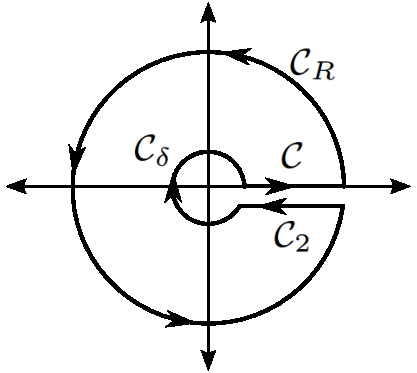
\includegraphics[width=0.3\textwidth]{./images/graph52}
    \caption{Representació gràfica dels camins sobre els quals s'integra la funció $x^{\alpha} R(x)$ a la demostració}
    \label{fig:graph52}
\end{figure}

\begin{sproof}
    \begin{align*}
    \begin{aligned}
        \int_{\mc{C} + \mc{C}_{R} + \mc{C}_{2} + \mc{C}_{\delta}} z^{\alpha}R(z) \diff z &= 2\pi i \sum_{z_{j} \notin \mbb{R}^{+}} \underset{z=z_{j}}{\operatorname{Res}} \lrpar{z^{\alpha}R(z)} \\
        &= \int_{\mc{C}} + \int_{\mc{C}_{R}} + \int_{\mc{C}_{2}} + \int_{\mc{C}_{\delta}} = I + I_{R} + I_{2} + I_{\delta}
    \end{aligned}
    \end{align*}
    Obserevem que volem trobar el valor de $I =\int_{\mc{C}} z^{a} R(z) \diff z$. Fent la parametrització $z = \rho\,e^{i\theta} \Rightarrow$
    \begin{itemize}
        \item $\displaystyle \abs{I_{R}} \leq \int_{0}^{2\pi} R^{\alpha} \abs{R\lrpar{R e^{i\theta}}} R \diff \theta = 2\pi \frac{R^{1+\alpha}}{R^{2+s}} \underset{R \to \infty}{\longrightarrow} 0$.
        \item $\displaystyle \abs{I_{\delta}} \leq \int_{2\pi}^{0} \delta^{\alpha} \abs{R \lrpar{\delta e^{i\theta}}} \delta \diff \theta = \int_{2\pi}^{0} \delta^{\alpha} \lrbra{\frac{1}{\delta} + \dots} \delta \diff \theta = - 2\pi \delta^{\alpha} \underset{\delta \to 0}{\longrightarrow} 0$.
        \item $\displaystyle I_{2} = \int_{R}^{\delta} e^{i2\pi} R\lrpar{r\,e^{i2\pi}} \lrpar{r e^{i2\pi - \varepsilon}}^{\alpha} \diff r = e^{i2\pi \alpha} \int_{R}^{\delta} r^{\alpha} R(r) \diff r = -e^{i2\pi \alpha} I$.
    \end{itemize}
    Llavors, tenim $\displaystyle I \lrpar{1-e^{i2\pi \alpha}} = 2\pi i \sum_{z_{j} \notin \mbb{R}^{+}} \underset{z=z_{j}}{\operatorname{Res}} \lrpar{z^{\alpha}R(z)}$.
\end{sproof}
